\section{Group -- Air Distribution}\label{group-air-distribution}

\subsection{AirLoopHVAC}\label{airloophvac}

Air loops along with zone equipment form the entire forced air heating and cooling system (air side). The main statement for defining an air loop is the \emph{AirLoopHVAC} object described here. As with the main plant and condenser statements, several of the items in the AirLoopHVAC object definition are actually names that refer to other objects in the input file. After the AirLoopHVAC object name, four such list pointers are encountered: for controllers, system availability, branches, and connectors. The Controller List defines how the air loop will respond due to various inputs (control signals). The Availability Manager List refers to methods for controlling when a system is operational. This may be as simple as a schedule to define when the system is shutdown. The Branch List lists the branches that comprise the primary air system. Finally, the Connector List lists the connections between the branches. The branches and connections together define the primary air system topology.

The only numeric input is the design primary air flow rate. This item is input just before the \hyperref[branchlist]{BranchList} name.

The next series of names refer to nodes for the various inlet and outlet points of the air loop. The air loop starts where the zone equipment ends. This is a single point consisting of the return air duct once all of the zone return air streams have been collected (if the loop has a return path). While in reality, there is really only one point, for clarity within the simulation components and consistency with the other HVAC loop sections, this point in the systems is defined as two points: one that resides with the zone equipment simulation and one that is acted upon by the air loop simulation. Both node names must be entered into the input file (if the loop has a return path), and both nodes must have unique names. Similarly, the end points of the air loop that also correspond to the beginning points of the zone equipment loop must also be defined. These consist of names referencing lists of up to three pairs of node names as shown below. Up to three air loop outlets are allowed to accommodate the simulation of three deck systems.

\paragraph{Schedules And Availability Manager}
Regarding component schedules, the general rule is don't schedule any components except the supply fan and the corresponding availability manager(s). Beyond that, every component should always be available and let the controls determine what runs or doesn't run. If a component other than the supply fan is scheduled off, then it will remain off even if the night cycle manager turns on the system.

\subsubsection{Inputs}\label{inputs-002}

\paragraph{Field: Name}

This field is a unique, user assigned name for a single instance of an AirLoopHVAC object. Any other object referencing this AirLoopHVAC will use this name.

\paragraph{Field: Controller List Name}\label{field-controller-list-name}

This field is the name of a ControllerList object. A Controller List is simply a list of controllers giving both controller name and type. This Controller List specifies all the controllers that will act on this primary air loop. The order of the controllers in the list is significant: controllers are simulated sequentially in the order given in the Controller List.

\paragraph{Field: Availability Manager List Name}\label{field-availability-manager-list-name}

This field is the name of a AvailabilityManagerList object. An Availability Manager List is a list of Availability Managers giving both Availability Manager type and name. The availability managers in the list apply to this primary air loop. That is, they determine when and if this air loop is on or off, overriding the control provided by the central fan on/off schedule.

\paragraph{Field: Design Supply Air Flow Rate}\label{field-design-supply-air-flow-rate}

This is the system primary air design volumetric flow rate in cubic meters per second.

\paragraph{Field: Branch List Name}\label{field-branch-list-name}

This field is the object name of a \hyperref[branchlist]{BranchList} object (see \hyperref[branchlist]{BranchList} and Branch). The \hyperref[branchlist]{BranchList} named here specifies all the branches composing the primary air system. These branches, together with the Connectors listed in the \hyperref[connectorlist]{ConnectorList}, define the primary air system topology.

\paragraph{Field: Connector List Name}\label{field-connector-list-name}

This field is the name of \hyperref[connectorlist]{ConnectorList} object. This \hyperref[connectorlist]{ConnectorList} object lists all the Connectors (by type and name) that are included in this primary air system. These Connectors, together with the Branches in the \hyperref[branchlist]{BranchList}, define the topology of the primary air system.

\paragraph{Field: Supply Side Inlet Node Name}\label{field-supply-side-inlet-node-name}

The name of the air entrance node of this primary air system. If this air loop has a return path, then this is the inlet node for return air for this air system. If this air loop does not have a return path, then this node is where outdoor air or other air enters the supply side.

\paragraph{Field: Demand Side Outlet Node Name}\label{field-demand-side-outlet-node-name}

The name of the air outlet node for the zone equipment group (\hyperref[zonehvacequipmentconnections]{ZoneHVAC:EquipmentConnections} objects) attached to the primary air system. This should be the outlet node of a \hyperref[airloophvaczonemixer]{AirLoopHVAC:ZoneMixer} or AirloopHVAC:ReturnPlenum in the \hyperref[airloophvacreturnpath]{AirLoopHVAC:ReturnPath} for the zone equipment group attached to this primary air system. Leave this field blank if this air loop does not have a return path.

\paragraph{Field: Demand Side Inlet Node Names}\label{field-demand-side-inlet-node-names}

This field can be the name of a node which is the air inlet node for the zone equipment group (see \hyperref[zonehvacequipmentconnections]{ZoneHVAC:EquipmentConnections} objects) attached to this primary air system. Or, this field can be the name of a node list containing one or more nodes (up to 3). These nodes should be the inlet nodes to the \hyperref[airloophvaczonesplitter]{AirLoopHVAC:ZoneSplitter} or \hyperref[airloophvacsupplyplenum]{AirLoopHVAC:SupplyPlenum} in each of the \hyperref[airloophvacsupplypath]{AirLoopHVAC:SupplyPath}s for the zone equipment groups attached to this primary air system. For single duct systems, there is only one node name in this list. For two and three duct systems, the order of the nodes in this list must correspond with the order of the nodes in the Supply Side Outlet Node Names list.

\paragraph{Field: Supply Side Outlet Node Names}\label{field-supply-side-outlet-node-names}

This field can be the name of a node which is the air outlet node for each supply duct of this primary air system. Or, this field can be the name of a node list containing one or more nodes (up to 3). The list can contain the names of up to three nodes. For single duct systems, there is only one node name in this list. For two and three duct systems, the order of the nodes in this list must correspond with the order of the nodes in the Demand Side Inlet Node Names list.

\paragraph{Field: Design Return Air Flow Fraction of Supply Air Flow}\label{design-return-air-flow-fraction-of-supply-air-flow}

This field specifies the design air loop return air flow rate as a fraction of the supply flow rate when there is no exhaust flow.  It may be used to set zero return air flow for a DOAS system or to model a pressurized system where the return flow is a fraction of the supply flow. The return air flow rate will never be greater than the current supply air flow rate multiplied by this fraction.  It may be less if there is unbalanced exhaust from any zones served by this airloop. The default is 1.0. If the air loop has no return path, then this field is ignored.

An example of this statement in an IDF is:

\begin{lstlisting}

AirLoopHVAC,
    Main Dual Duct Air Loop,           !- Name
    Dual Duct System 1 Controllers,    !- Controller List Name
    Dual Duct System 1 Schedule List , !- Availability Manager List Name
    1.3 ,                              !- Design Supply Air Flow Rate {m3/s}
    Dual Duct Air Loop Branches ,      !- Branch List Name
    Dual Duct Connectors ,             !- Connector List Name
    Supply Fan Inlet Node ,            !- Supply Side Inlet Node Name
    Return Air Mixer Outlet ,          !- Demand Side Outlet Node Name
    Zone Equipment Inlet Node List ,   !- Demand Side Inlet Node Names
    Air Loop Outlet Node List,         !- Supply Side Outlet Node Names
    1.0;                               !- Design Return Air Flow Fraction of Supply Air Flow
\end{lstlisting}

\subsubsection{Outputs}\label{outputs-001}

\begin{itemize}
\item
  HVAC,Average,Air System Simulation Cycle On Off Status
\item
  HVAC,Sum,HVAC System Solver Iteration Count {[]}
\item
  HVAC,Sum,Air System Solver Iteration Count {[]}
\item
  HVAC,Sum,Air System Simulation Maximum Iteration Count {[]}
\item
  HVAC,Sum,Air System Simulation Iteration Count {[]}
\item
  HVAC,Sum,Air System Component Model Simulation Calls {[]}
\end{itemize}

\paragraph{Air System Simulation Cycle On Off Status}\label{air-system-simulation-cycle-on-off-status}

This field is the availability status of an AirLoopHVAC. This status flag is a result of the calculations made by the System Availability Manager(s) listed in a System Availability Manager List. When a single availability manager is used in a System Availability Manager List, this is also the availability status reported by the specific availability manager (Ref. System Availability Manager Outputs). When multiple availability managers are used in a System Availability Manager List, the loop availability status is determined by the rules associated with AirLoopHVACs (see rules described for Group -- System Availability Managers). The control status outputs are represented using integers 0 through 3.. These integers represent \emph{NoAction} (0), \emph{ForceOff} (1), \emph{CycleOn} (2), and \emph{CycleOnZoneFansOnly} (3). Since the status output is averaged, the output result may not correspond to the values described here when output variable frequencies other than detailed are used. Use the ``detailed'' reporting frequency (Ref. Output:Variable object) to view the availability status at each simulation timestep.

\paragraph{HVAC System Solver Iteration Count {[]}}\label{hvac-system-solver-iteration-count}
This field reports the total number of HVAC System solver iterations in the current system time step or the maximum iterations possible for this solver if the simulation has not yet converged before it reached the maximum iterations.

\paragraph{Air System Solver Iteration Count {[]}}\label{air-system-solver-iteration-count}
This field reports the total number of Air System solver iterations in the current system time step or the maximum iterations possible for this solver if the simulation has not yet converged before it reached the maximum iterations.

\paragraph{Air System Simulation Maximum Iteration Count {[]}}\label{air-system-simulation-maximum-iteration-count}
This field reports the maximum number of iterations possible for an Air System simulation.

\paragraph{Air System Simulation Iteration Count {[]}}\label{air-system-simulation-iteration-count}
This field reports the total number of Air System iterations in the current system time step or the maximum iterations possible for this solver if the simulation has not yet converged before it reached the maximum iterations.

\paragraph{Air System Component Model Simulation Calls {[]}}\label{air-system-component-model-simulation-calls}

These variables are simply counters of how many iterations were executed. The count for any given HVAC time step will be the iterations executed before convergence was achieved, or the max allowed in which case the simulation throws a warning and proceeds to the next time step.

\subsubsection{Outputs}\label{outputs-1-001}

This section provides more detailed information on the reporting available for outdoor air ventilation.~ Sixteen cooling and heating load variables and eight energy summary variables are available that report the impact of system outdoor air on zone loads, system demand and total energy use. The representative air system shown in the diagram below shows outdoor air (OA), return air (RA), supply air (SA) and mixed air (MA).

\begin{figure}[hbtp] % fig 90
\centering
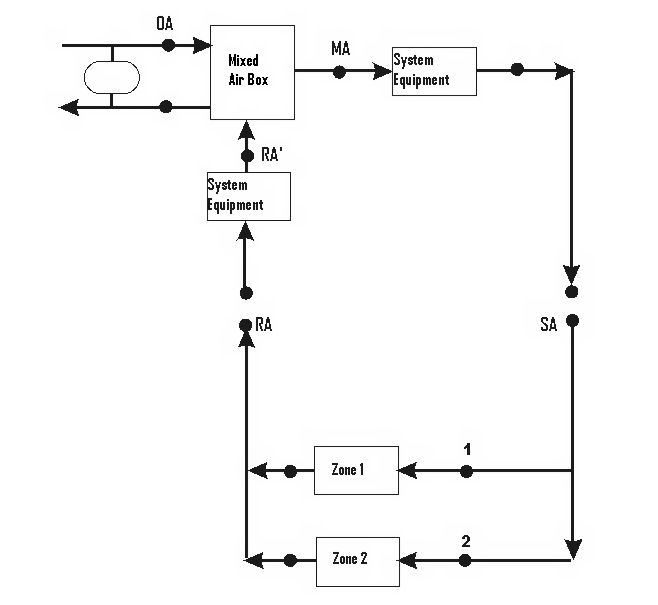
\includegraphics[width=0.9\textwidth, height=0.9\textheight, keepaspectratio=true]{media/image209.png}
\caption{Example System for Ventilation Loads Report \protect \label{fig:example-system-for-ventilation-loads-report}}
\end{figure}

The overall effect of outdoor air on the system shown above can be summarized by considering the mixing box. In this system, part or all of the return air is replaced by outdoor air. The presence of any heat recovery will already be taken into account and thus will automatically be accounted for by using the outdoor air inlet conditions to the mixing box (point OA in the diagram) rather than actual outdoor air conditions. Thus, the overall energy impact of outdoor air (ventilation) on a particular system can be evaluated by multiplying the outdoor air mass flow rate by the enthalpy difference between the outdoor air entering the mixing box (OA) and the return air entering the mixing box (RA') as shown in the following equation.

\begin{equation}
{\dot q_{OA}} = {\dot m_{OA}}\left( {{h_{OA}} - {h_{RA'}}} \right) = {\dot m_{sys}}\left( {{h_{MA}} - {h_{RA'}}} \right)
\end{equation}

\paragraph{Ventilation Flow Outputs}\label{ventilation-flow-outputs}

The fresh air flow into each zone are reported using the ventilation flow output variables. The total outdoor air flow in a primary air system is divided to each zone based on the fraction of flow each zone is supplied. There are six variables which deals with the mechanical ventilation flow reporting. Those six variables are:

\paragraph{Zone Mechanical Ventilation Mass Flow Rate {[}kg/s{]}}\label{zone-mechanical-ventilation-mass-flow-rate-kgs}

Reports the average outdoor air mass flow rate to any zone over the reporting interval.

\paragraph{Zone Mechanical Ventilation Mass {[}kg{]}}\label{zone-mechanical-ventilation-mass-kg}

Reports the total outdoor air mass that has been supplied to any zone over the reporting interval.

\paragraph{Zone Mechanical Ventilation Standard Density Volume Flow Rate {[}m3/s{]}}\label{zone-mechanical-ventilation-standard-density-volume-flow-rate-m3s}

Reports the average outdoor air volume flow rate to any zone over the reporting interval, calculated using a standard density for air. Standard density in EnergyPlus corresponds to 20ºC drybulb, dry air, and nominally adjusted for elevation.

\paragraph{Zone Mechanical Ventilation Standard Density Volume {[}m3{]}}\label{zone-mechanical-ventilation-standard-density-volume-m3}

Reports the total outdoor air volume that has been supplied to a zone over the reporting interval, calculated using a standard density for air.~ Standard density in EnergyPlus corresponds to 20ºC drybulb, dry air, and nominally adjusted for elevation.

\paragraph{Zone Mechanical Ventilation Current Density Volume Flow Rate {[}m3/s{]}}\label{zone-mechanical-ventilation-current-density-volume-flow-rate-m3s}

Reports the average outdoor air volume flow rate to any zone over the reporting interval, calculated using the current density for zone air.

\paragraph{Zone Mechanical Ventilation Current Density Volume {[}m3{]}}\label{zone-mechanical-ventilation-current-density-volume-m3}

Reports the total outdoor air volume that has been supplied to a zone over the reporting interval, calculated using the current density for zone air.

\paragraph{Zone Mechanical Ventilation Air Changes per Hour {[}ach{]}}\label{zone-mechanical-ventilation-air-changes-per-hour-ach}

Reports the air changes per hour in the zone due to the outside fresh air supplied by mechanical ventilation system.

The example syntax below shows the basic ventilation flow variables reported on an hourly basis.

\begin{itemize}
\item
  Output:Variable,*,Zone Mechanical Ventilation Mass Flow Rate,Hourly;
\item
  Output:Variable,*,Zone Mechanical Ventilation Mass,Hourly;
\item
  Output:Variable,*,Zone Mechanical Ventilation Standard Density Volume Flow Rate,Hourly;
\item
  Output:Variable,*,Zone Mechanical Ventilation Standard Density Volume,Hourly;
\item
  Output:Variable,*,Zone Mechanical Ventilation Current Density Volume Flow Rate,Hourly;
\item
  Output:Variable,*,Zone Mechanical Ventilation Current Density Volume,Hourly;
\item
  Output:Variable,*, Zone Mechanical Ventilation Air Changes per Hour,Hourly;
\end{itemize}

\paragraph{Ventilation Load Reports}\label{ventilation-load-reports}

The impact of system outdoor air on a particular zone may be calculated by summing the mass flow weighted \({\dot q_{OA}}\) ~over the supply air paths (both cooling and heating) serving the zone as follows:

\begin{equation}
{\dot q_{OA,Zone\;1}} = \sum\limits_{n = 1}^{AirPathNum} {{{\dot q}_{OA}}\frac{{{{\dot m}_n}}}{{{{\dot m}_{sys}}}}}
\end{equation}

Four output variables each for cooling and heating report the impact of the ventilation air on the zone load in the absence of ventilation air system interactions. The ventilation load output variables are:

\paragraph{Zone Mechanical Ventilation Cooling Load Increase Due to Overheating Energy {[}J{]}}\label{zone-mechanical-ventilation-cooling-load-increase-due-to-overheating-energy-j}

\paragraph{Zone Mechanical Ventilation Heating Load Increase Due to Overcooling Energy {[}J{]}}\label{zone-mechanical-ventilation-heating-load-increase-due-to-overcooling-energy-j}

The cooling/heating load that would occur once ventilation air met the zone cooling/heating load and continued to overcool/overheat the zone. No system effects are accounted for.

\paragraph{Zone Mechanical Ventilation Cooling Load Decrease Energy {[}J{]}}\label{zone-mechanical-ventilation-cooling-load-decrease-energy-j}

\paragraph{Zone Mechanical Ventilation Heating~ Load Decrease{[}J{]}}\label{zone-mechanical-ventilation-heating-load-decreasej}

The decrease in zone cooling/heating load that would occur as a result of ventilation air introduced directly into the zone. No system effects are accounted for.

\paragraph{Zone Mechanical Ventilation No Load Heat Removal Energy {[}J{]}}\label{zone-mechanical-ventilation-no-load-heat-removal-energy-j}

\paragraph{Zone Mechanical Ventilation No Load Heat Addition Energy {[}J{]}}\label{zone-mechanical-ventilation-no-load-heat-addition-energy-j}

The addition or removal of heat to a zone with no load. The heat addition or removal is due to mechanical ventilation while the zone thermostat is in the deadband.

To summarize:

\textbf{Cooling:}

\textbf{\emph{1.~~~~Zone Mechanical Ventilation No Load Heat Removal Energy {[}J{]}}}

Cooling that would be provided directly to zone by ventilation air. Ventilation occurred with no zone load.

\textbf{\emph{2.~~~~Zone Mechanical Ventilation Cooling Load Increase Energy {[}J{]}}}

The increase in zone cooling load that would occur as a result of ventilation air introduced directly into the zone. No system effects are accounted for.

\textbf{\emph{3.~~~~Zone Mechanical Ventilation Cooling Load Increase Due to Overheating Energy {[}J{]}}}

The cooling load that would occur once ventilation air met the zone heating load and continued to overheat the zone. No system effects are accounted for.

\textbf{\emph{4.~~~~Zone Mechanical Ventilation Cooling Load Decrease Energy {[}J{]}}}

The decrease in zone cooling load that would occur as a result of ventilation air introduced directly into the zone. No system effects are accounted for.

\textbf{Heating:}

\textbf{\emph{1.~~~~Zone Mechanical Ventilation No Load Heat Addition Energy {[}J{]}}}

Heating that would be provided directly to zone by ventilation air. Ventilation occurred with no zone load.

\textbf{\emph{2.~~~~Zone Mechanical Ventilation Heating Load Increase Energy {[}J{]}}}

The increase in zone heating load that would occur as a result of ventilation air introduced directly into the zone. No system effects are accounted for.

\textbf{\emph{3.~~~~Zone Mechanical Ventilation Heating Load Increase Due to Overcooling Energy {[}J{]}}}

The heating load that would occur once ventilation air met the zone cooling load and continued to overcool the zone. No system effects are accounted for.

\textbf{\emph{4.~~~~Zone Mechanical Ventilation Heating Load Decrease Energy {[}J{]}}}

The decrease in zone heating load that would occur as a result of ventilation air introduced directly into the zone. No system effects are accounted for.

The output variables are calculated by comparing the zone ventilation load with the zone cooling or heating load.~ `Ventilation cooling' decreases the zone cooling load until the cooling load has been eliminated. The remaining `ventilation cooling' is reported as `overcooling'. `Overheating' is calculated in the same manner. The actual system operation, which determines whether or not an `overcooling' or `overheating' load actually results in increased energy consumption, is not considered in the calculation of these output variables.

The ventilation zone load output variables are shown in Table~\ref{table:ventilation-load-output-variables}. The variables report the maximum potential ``cost'' or ``benefit'' of ventilation air introduced directly into the zone.

% table 24
\begin{longtable}[c]{p{1.5in}p{1.5in}p{1.5in}p{1.5in}}
\caption{Ventilation Load Output Variables \label{table:ventilation-load-output-variables}} \tabularnewline
\toprule
 & No Zone Load & Zone Cooling Load & Zone Heating Load \tabularnewline
\midrule
\endfirsthead

\caption[]{Ventilation Load Output Variables} \tabularnewline
\toprule
 & No Zone Load & Zone Cooling Load & Zone Heating Load \tabularnewline
\midrule
\endhead

Ventilation Cooling & Zone Mechanical Ventilation No Load Heat Removal Energy & Zone Mechanical Ventilation Cooling Load Decrease Energy & Zone Mechanical Ventilation Heating Load Increase Energy \tabularnewline
Zone Mechanical Ventilation Heating Load Increase Due to Overcooling Energy \tabularnewline
Ventilation Heating & Zone Mechanical Ventilation No Load Heat Addition Energy & Zone Mechanical Ventilation Cooling Load Increase Energy & Zone Mechanical Ventilation Heating Load Decrease Energy \tabularnewline
Zone Mechanical Ventilation Cooling Load Increase Due to Overheating Energy \tabularnewline
\bottomrule
\end{longtable}

The example syntax below shows the basic ventilation load variables reported on a monthly basis.

\begin{itemize}
\item
  ~ Output:Variable,*,Zone Mechanical Ventilation Heating Load Increase Energy,monthly;
\item
  ~ Output:Variable,*,Zone Mechanical Ventilation Heating Load Decrease Energy,monthly;
\item
  ~ Output:Variable,*,Zone Mechanical Ventilation No Load Heat Addition Energy,monthly;
\item
  ~ Output:Variable,*,Zone Mechanical Ventilation Cooling Load Increase Energy,monthly;
\item
  ~ Output:Variable,*,Zone Mechanical Ventilation Cooling Load Decrease Energy,monthly;
\item
  ~ Output:Variable,*,Zone Mechanical Ventilation No Load Heat Removal Energy,monthly;
\end{itemize}

Reporting on a timestep or hourly level would produce a detailed report with variables intermingled with the other output variables that might be requested in the input file.

Another method will more easily encapsulate the report:

\begin{lstlisting}

OutputControl:Table:Style, HTML;     !- ColumnSeparator


  Output:Table:Monthly,
    Ventilation Loads,       !- Name
    ,                        !- DigitsAfterDecimal
  Zone Mechanical Ventilation No Load Heat Removal Energy,
           SumOrAverage,
  Zone Mechanical Ventilation Cooling Load Increase Due to Overheating Energy,
           SumOrAverage,
  Zone Mechanical Ventilation Cooling Load Decrease Energy,
           SumOrAverage,
  Zone Mechanical Ventilation Cooling Load Increase Energy,
           SumOrAverage,
  Zone Mechanical Ventilation No Load Heat Addition Energy,
           SumOrAverage,
  Zone Mechanical Ventilation Heating Load Increase Due to Overcooling Energy,
           SumOrAverage,
  Zone Mechanical Ventilation Heating Load Decrease Energy,
           SumOrAverage,
  Zone Mechanical Ventilation Heating Load Increase Energy,
           SumOrAverage;
\end{lstlisting}

This combination will report the ventilation loads on a monthly basis in a HTML style report that can be easily read in a web browser. Review the Output:Table:Monthly object for other methods of display or further options on this report item.

\subsection{Systems Level Reporting}\label{systems-level-reporting}

Most output variables are a single entity reporting. Meters are a combination of like variables -- specifically for Energy Consumption. This section introduces a slightly different concept -- where output variables described herein are a combination of several similar items -- specifically targeted at HVAC/System level reporting. This reporting is coupled with an Air Loop (ref: \hyperref[airloophvac]{AirLoopHVAC})

All items shown in this section are typical ``output variables'' and can be reported with the \hyperref[outputvariable]{Output:Variable} object.

Or, as is shown by example here, perhaps a more readable form is to generate them in Tabular Form with the ``\hyperref[outputtablemonthly]{Output:Table:Monthly}'' object.

\begin{figure}[hbtp] % fig 91
\centering
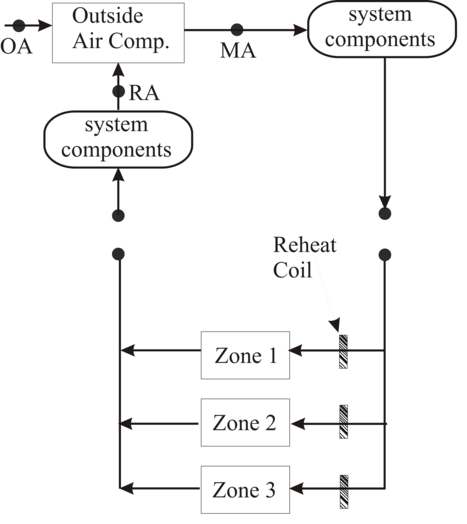
\includegraphics[width=0.9\textwidth, height=0.9\textheight, keepaspectratio=true]{media/image213.png}
\caption{View of System Level Reporting \protect \label{fig:view-of-system-level-reporting}}
\end{figure}

\subsection{System Loads Outputs}\label{system-loads-outputs}

In this category, the total system load is reported. Two aspects are reported here: Heating and Cooling. The following two variables report the heat energy that system components (including packaged equipment, fans, main coils, reheat coils, humidifiers, desiccant dehumidifiers, evaporative coolers and heat exchangers) add or remove from the air loop. Each variable within these grouping wil

\subsubsection{Air System Total Heating Energy}\label{air-system-total-heating-energy}

Heat Addition to the Air Loop (Sum of all components) in Joules

\subsubsection{Air System Total Cooling Energy}\label{air-system-total-cooling-energy}

Heat Removal from the Air Loop (Sum of all components) in Joules

In `\hyperref[outputtablemonthly]{Output:Table:Monthly}' format shown below.

\begin{lstlisting}

  OutputControl:Table:Style,HTML;

    Output:Table:Monthly,
      System Loads,       !- Name
      ,                        !- DigitsAfterDecimal
      Air System Total Heating Energy,  SumOrAverage,
      Air System Total Cooling Energy,  SumOrAverage;
\end{lstlisting}

\subsection{System Energy Use Outputs}\label{system-energy-use-outputs}

System Energy Use consists of six output variables that report the total energy (in Joules) and water consumption (in m\(^{3}\)) for all system components and including packaged equipment, fans, main coils, reheat coils, humidifiers, desiccant dehumidifiers, and evaporative coolers. The output variables shown below show hot and cold water, steam, electric and gas energy. Hot and cold water energy includes all `district cooling' and `district heating' energy.

\subsubsection{Air System Hot Water Energy}\label{air-system-hot-water-energy}

Hot Water Consumption for the system (Joules).

\subsubsection{Air System Steam Energy}\label{air-system-steam-energy}

Steam Consumption for the system (Joules).

\subsubsection{Air System Chilled Water Energy}\label{air-system-chilled-water-energy}

Chilled Water Consumption for the system (Joules).

\subsubsection{Air System Electricity Energy}\label{air-system-electric-energy}

Electric Consumption for the system (Joules).

\subsubsection{Air System NaturalGas Energy}\label{air-system-gas-energy}

Natural Gas Consumption for the system (Joules).

\subsubsection{Air System Propane Energy}

Propane Consumption for the system (Joules).

\subsubsection{Air System Water Volume}\label{air-system-water-volume}

Water Consumption for the system (humidifiers and evaporative coolers) (m3).

The Standard reports file includes these variables reporting in the Tabular report form as ``Air Loop System Energy and Water Use''.

\begin{lstlisting}

  OutputControl:Table:Style,HTML;

    Output:Table:Monthly,
      Air Loop System Energy and Water Use,       !- Name
      ,                        !- DigitsAfterDecimal
      Air System Hot Water Energy ,  SumOrAverage,
      Air System Steam Energy ,  SumOrAverage,
      Air System Chilled Water Energy,  SumOrAverage,
      Air System Electricity Energy,  SumOrAverage,
      Air System NaturalGas Energy,  SumOrAverage,
      Air System Water Volume,  SumOrAverage;
\end{lstlisting}

\subsection{System Component Loads Outputs}\label{system-component-loads-outputs}

Reporting System Component Loads shows the energy transferred to or extracted from the air loop by system component type. Fans, Cooling Coils, Heating Coils, Heat exchangers, humidifiers, evaporative coolers, and desiccant dehumidifiers show heat transfer rates in Joules. The components may be located in outdoor air systems bundled with packaged equipment or specified as stand-alone components. The reporting accounts for both main branch and reheat coils.

The Standard reports file includes these variables reporting in the Tabular report form as ``Air Loop System Component Loads''.

\begin{lstlisting}

  OutputControl:Table:Style,HTML;


    Output:Table:Monthly,
      Air Loop System Component Loads,       !- Name
      ,                        !- DigitsAfterDecimal
      Air System Fan Air Heating Energy,  SumOrAverage,
      Air System Cooling Coil Total Cooling Energy,  SumOrAverage,
      Air System Heating Coil Total Heating Energy,  SumOrAverage,
      Air System Heat Exchanger Total Heating Energy,  SumOrAverage,
      Air System Heat Exchanger Total Cooling Energy,  SumOrAverage,
      Air System Humidifier Total Heating Energy,  SumOrAverage,
      Air System Evaporative Cooler Total Cooling Energy,  SumOrAverage,
      Air System Desiccant Dehumidifier Total Cooling Energy,  SumOrAverage;
\end{lstlisting}

\subsubsection{Air System Fan Air Heating Energy}\label{air-system-fan-air-heating-energy}

Energy added to the air loop by Fans (Joules)

\subsubsection{Air System Cooling Coil Total Cooling Energy}\label{air-system-cooling-coil-total-cooling-energy}

Energy removed from air loop by Cooling Coils (Joules)

\subsubsection{Air System Heating Coil Total Heating Energy}\label{air-system-heating-coil-total-heating-energy}

Energy added to air loop by Heating Coils (Joules)

\subsubsection{Air System Heat Exchanger Total Heating Energy}\label{air-system-heat-exchanger-total-heating-energy}

Energy added to air loop by air-to-air heat recovery heat exchangers (Joules)

\subsubsection{Air System Heat Exchanger Total Cooling Energy}\label{air-system-heat-exchanger-total-cooling-energy}

Energy removed from air loop by air-to-air heat recovery heat exchangers (Joules)

\subsubsection{Air System Humidifier Total Heating Energy}\label{air-system-humidifier-total-heating-energy}

Energy added to air loop by humidifiers (Joules)

\subsubsection{Air System Evaporative Cooler Total Cooling Energy}\label{air-system-evaporative-cooler-total-cooling-energy}

Energy removed from air loop by evaporative coolers (Joules)

\subsubsection{Air System Desiccant Dehumidifier Total Cooling Energy}\label{air-system-desiccant-dehumidifier-total-cooling-energy}

Energy removed from air loop by desiccant dehumidifiers (Joules)

\subsubsection{Air System Solar Collector Total Heating Energy}\label{air-system-solar-collector-total-heating-energy}

Energy added to air loop by solar collectors (Joules)

\subsubsection{Air System Solar Collector Total Cooling Energy}\label{air-system-solar-collector-total-cooling-energy}

Energy removed from air loop by solar collectors (Joules)

\subsubsection{Air System User Defined Air Terminal Total Heating Energy}\label{air-system-user-defined-air-terminal-total-heating-energy}

Energy added to air loop by user defined air terminal units (Joules)

\subsubsection{Air System User Defined Air Terminal Total Cooling Energy}\label{air-system-user-defined-air-terminal-total-cooling-energy}

Energy removed from air loop by user defined air terminal units (Joules)

\subsection{System Component Energy Use Outputs}\label{system-component-energy-use-outputs}

Reporting System Component Energy Use consists of eleven output variables that report the total energy consumption (in Joules) of system components by energy type and coil type. Electric energy consumption is reported for fans, heating and cooling coils in packaged (DX) systems, electric resistance heating coils, humidifiers, evaporative coolers and desiccant dehumidifiers.

\subsubsection{Air System Fan Electricity Energy}\label{air-system-fan-electric-energy}

Electric consumption for fans. (Joules)

\subsubsection{Air System Heating Coil Hot Water Energy}\label{air-system-heating-coil-hot-water-energy}

Consumption for heating coil hot water (both purchased and plant supplied) (Joules)

\subsubsection{Air System Cooling Coil Chilled Water Energy}\label{air-system-cooling-coil-chilled-water-energy}

Consumption for cooling coil chilled water (both purchased and plant supplied) (Joules)

\subsubsection{Air System DX Heating Coil Electricity Energy}\label{air-system-dx-heating-coil-electric-energy}

Compressor plus condenser fan electricity use. (Joules)

\subsubsection{Air System DX Cooling Coil Electricity Energy}\label{air-system-dx-cooling-coil-electric-energy}

Compressor plus condenser fan electricity use. (Joules)

\subsubsection{Air System Heating Coil Electricity Energy}\label{air-system-heating-coil-electric-energy}

Electricity consumption for the heating coil. (Joules)

\subsubsection{Air System Heating Coil NaturalGas Energy}\label{air-system-heating-coil-gas-energy}

Natural Gas consumption for the heating coil. (Joules)

\subsubsection{Air System Heating Coil Propane Energy}\label{air-system-heating-coil-propane-energy}

Propane consumption for the heating coil. (Joules)

\subsubsection{Air System Heating Coil Steam Energy}\label{air-system-heating-coil-steam-energy}

Steam consumption for the heating coil (steam coils). (Joules)

\subsubsection{Air System Humidifier Electricity Energy}\label{air-system-humidifier-electric-energy}

Electricity consumption for the humidifiers. (Joules)

\subsubsection{Air System Evaporative Cooler Electricity Energy}\label{air-system-evaporative-cooler-electric-energy}

Electricity consumption for the evaporative coolers. (Joules)

\subsubsection{Air System Desiccant Dehumidifier Electricity Energy}\label{air-system-desiccant-dehumidifier-electric-energy}

Electricity consumption for the desiccant dehumidifiers. (Joules)

The Standard reports file includes these variables reporting in the Tabular report form as ``Air Loop System Component Energy Use''.

\begin{lstlisting}

  OutputControl:Table:Style,HTML;


    Output:Table:Monthly,
      Air Loop System Component Energy Use,       !- Name
      ,                        !- DigitsAfterDecimal
      Air System Fan Electricity Energy,  SumOrAverage,
      Air System Heating Coil Hot Water Energy,  SumOrAverage,
      Air System Cooling Coil Chilled Water Energy,  SumOrAverage,
      Air System DX Heating Coil Electricity Energy,  SumOrAverage,
      Air System DX Cooling Coil Electricity Energy,  SumOrAverage,
      Air System Heating Coil Electricity Energy,  SumOrAverage,
      Air System Heating Coil Gas Energy,  SumOrAverage,
      Air System Heating Coil Steam Energy,  SumOrAverage,
      Air System Humidifier Electricity Energy,  SumOrAverage,
      Air System Evaporative Cooler Electricity Energy,  SumOrAverage,
      Air System Desiccant Dehumidifier Electricity Energy,  SumOrAverage;
\end{lstlisting}

\subsection{Overall Air Loop Syntax}\label{overall-air-loop-syntax}

A map for Air Loop input syntax is shown in the following diagram.

\begin{figure}[hbtp] % fig 92
\centering
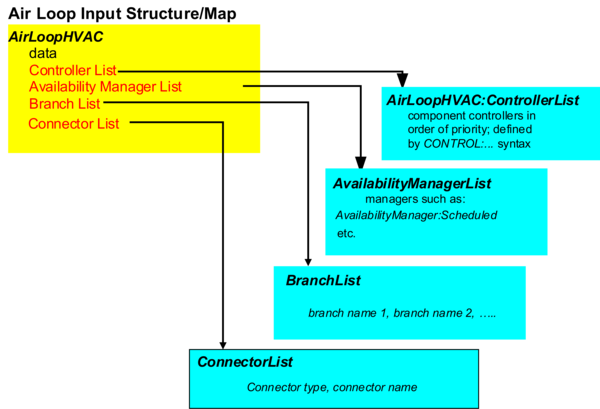
\includegraphics[width=0.9\textwidth, height=0.9\textheight, keepaspectratio=true]{media/image214.png}
\caption{Air Loop Input Syntax Map \protect \label{fig:air-loop-input-syntax-map}}
\end{figure}

\subsection{AirLoopHVAC:ControllerList}\label{airloophvaccontrollerlist}

The syntax for the AirLoopHVAC:ControllerList definition is shown below. As with other lists in EnergyPlus input, the object title and identifying name are followed by type-name pairs. In this case, the types are controller types. The order in which controllers appear on this list also define the priority as described below. The identifying name refers back to the name recorded in the \hyperref[airloophvac]{AirLoopHVAC} statement.

\subsubsection{Inputs}\label{inputs-1-002}

\paragraph{Field: Name}\label{field-name-1-001}

The user designated unique name of an instance of a Controller List. Any object referencing this Controller List will do so using this name.

\paragraph{Field Set (Object Type, Controller Name) up to 8}\label{field-set-object-type-controller-name-up-to-8}

After the identifying name, input for the controller list consists of up to 8 pairs of data items: a controller type and a controller name. The first controller listed has the highest priority, the second the second highest priority, and so forth.

\paragraph{Field: Controller \textless{}x\textgreater{} Object Type}\label{field-controller-x-object-type}

The type of~ controller. This should be a key word defining a class of controllers such as \hyperref[controllerwatercoil]{Controller:WaterCoil}.

\paragraph{Field: Controller \textless{}x\textgreater{} Name}\label{field-controller-x-name}

The name of a controller object (such as a \hyperref[controllerwatercoil]{Controller:WaterCoil}) defined elsewhere in the input file.

An example of this statement in an IDF is:

\begin{lstlisting}

AirLoopHVAC:ControllerList,
             Dual Duct System 1 Controllers,
             Controller:WaterCoil, Main Cooling Coil Controller,
             Controller:WaterCoil, Main Heating Coil Controller;
\end{lstlisting}

\subsection{AvailabilityManagerAssignmentList}\label{availabilitymanagerassignmentlist}

The AvailabilityManagerAssignmentList defines the applicable managers used for an \hyperref[airloophvac]{AirLoopHVAC} or \hyperref[plantloop]{PlantLoop}. The priority of availability managers is based on a set of rules and are specific to the type of loop. The output from each Availability Manager is an availability status flag. This flag can have the values \emph{NoAction}, \emph{ForceOff}, \emph{CycleOn}, or \emph{CycleOnZoneFansOnly} (used only for air loops). The availability status flags for the Availability Managers referenced by an air or plant loop are used to set the availability status flag for each loop. For the air loops, \emph{ForceOff} takes precedence: if any of the loop's availability managers are showing status \emph{ForceOff}, the loop status will be \emph{ForceOff}. Next in precedence is \emph{CycleOnZoneFansOnly,} followed by \emph{CycleOn}, and \emph{NoAction}. For the plant loops, there is no precedence among the Availability Manager status flag values. Instead, the first availability manager giving a status flag value other than \emph{NoAction} sets the status for the loop. The Availability Managers are executed in Availability Manager List order.

Special rules also apply for which managers may be listed in an Availability Manager list. The Hybrid Ventilation Control Manager (object: \hyperref[availabilitymanagerhybridventilation]{AvailabilityManager:HybridVentilation}) is a special type of manager and is never specified in an Availability Manager List (it is used stand-alone for a specific air loop). All other types of availability managers may be listed in the Availability Manager List used for \hyperref[airloophvac]{AirLoopHVAC}s. For Plant Loops, the Night Cycle and Night Ventilation managers (objects: \hyperref[availabilitymanagernightcycle]{AvailabilityManager:NightCycle} ~and \hyperref[availabilitymanagernightventilation]{AvailabilityManager:NightVentilation}) are not allowed in the Availability Manager List.

\subsubsection{Inputs}\label{inputs-2-002}

\paragraph{Field: Name}\label{field-name-2-001}

The name of the AvailabilityManagerAssignmentList ~object. This is referenced by \hyperref[airloophvac]{AirLoopHVAC} and \hyperref[plantloop]{PlantLoop} objects.

\paragraph{Field Set (Availability Manager Object Type, Name)}\label{field-set-availability-manager-object-type-name}

Managers are listed by pairs of data items:~ \emph{Availability Manager Object Type} and \emph{Availability Manager Name}. The managers are simulated down the list and calculate a control status for use by the \hyperref[airloophvac]{AirLoopHVAC} or \hyperref[plantloop]{PlantLoop}. The priority of each manager used for a specific loop is based on the rules described above. Availability managers are not currently used for condenser loops. The availability managers, along with the \hyperref[airloophvac]{AirLoopHVAC} and \hyperref[plantloop]{PlantLoop} object, report the control status calculated each simulation timestep. These output variables can be used to prioritize the managers according to the required control strategy. Six managers are accomodated in the list by default, however, this IDD specification is extensible. Additional pairs may be added by directly editing the IDD.

\paragraph{Field: Availability Manager \textless{}x\textgreater{} Object Type}\label{field-availability-manager-x-object-type}

The key word defining the type of manager, e.g.~\hyperref[availabilitymanagernightcycle]{AvailabilityManager:NightCycle}.

\paragraph{Field: Availability Manager\textless{}x\textgreater{}~ Name}\label{field-availability-managerx-name}

The name of a AvailabilityManager object defined elsewhere in the input file.

An example of this statement in an IDF is:

\begin{lstlisting}

AvailabilityManagerAssignmentList,
    Collector Loop Availability Manager List,  !- Name
    AvailabilityManager:HighTemperatureTurnOff,    !- System Availability Manager Type 1
    High Temperature Turn Off Availability Manager,  !- System Availability Manager Name 1
    AvailabilityManager:LowTemperatureTurnOn ,     !- System Availability Manager Type 2
    Low Temperature Turn On Availability Manager,  !- System Availability Manager Name 2
    AvailabilityManager:DifferentialThermostat,    !- System Availability Manager Type 3
    Differential Thermostat Availability Manager;  !- System Availability Manager Name 3
\end{lstlisting}

\subsection{AirLoopHVAC:OutdoorAirSystem}\label{airloophvacoutdoorairsystem}

The Outside Air System (object AirLoopHVAC:OutdoorAirSystem) is a subsystem of an \hyperref[airloophvac]{AirLoopHVAC}. It handles the mixed air portion of the primary air system: the system relief air, the outside air inlet, and any components and controllers associated with the system relief air and outside air streams. From the perspective of the primary air loop the Outside Air System is treated as a single component. As a subsystem, it can contain one or more components and controllers.

The input for the Outside Air System consists of a system name, a controller list name, an equipment list name, and an availability manager list name. The controller list simply lists, by type and unique name, all the controllers in the subsystem. The controllers will be simulated in list order. The equipment list lists all the components in the subsystem, by type and name. The equipment is simulated in list order. Finally, the availability manager list gives the type and name of the availability managers used by the subsystem.

The equipment inlet/outlet must be sequential with no loops - the simulation can only handle a straight-through air path, both on the primary air side and on the secondary air side, if any. Heat exchanger secondary air inlets need to be independent of the primary air stream -- usually relief air is used.

The Outside Air System (object AirLoopHVAC:OutdoorAirSystem) can also be defined as a subsystem of an \hyperref[airloophvacdedicatedoutdoorairsystem]{AirLoopHVAC:DedicatedOutdoorAirSystem}. When this subsystem is referred in AirLoopHVAC:DedicatedOutdoorAirSystem, the \hyperref[controlleroutdoorair]{Controller:OutdoorAir} can not be listed in the \hyperref[airloophvaccontrollerlist]{AirLoopHVAC:ControllerList}, because the outdoor air flow rate will not be determined by Controller:OutdoorAir. Instead, the outdoor air flow rate will be specified by \hyperref[airloophvacdedicatedoutdoorairsystem]{AirLoopHVAC:DedicatedOutdoorAirSystem}.  In addition, the \hyperref[outdoorairmixer]{OutdoorAir:Mixer} will not be allowed in the \hyperref[airloophvacoutdoorairsystemequipmentlist]{AirLoopHVAC:OutdoorAirSystem:EquipmentList} as a component, because no mix is needed due to 100\% outdoor incoming airflow determined by AirLoopHVAC:DedicatedOutdoorAirSystem.

\subsubsection{Inputs}\label{inputs-3-001}

\paragraph{Field: Name}\label{field-name-3-001}

The unique, user assigned name for a single instance of an Outside Air System. Any other object referencing this Outside Air System will use this name.

\paragraph{Field: Name: Controller List Name}\label{field-name-controller-list-name}

This field is the name of a \hyperref[airloophvaccontrollerlist]{AirLoopHVAC:ControllerList} object. A \hyperref[airloophvaccontrollerlist]{AirLoopHVAC:ControllerList} is simply a list of controllers giving both controller name and type. This Controller List specifies all the controllers that will act on this outside air system. The order of the controllers in the list is significant: controllers are simulated sequentially in the order given in the Controller List. Typically the Controller List would contain a \hyperref[controlleroutdoorair]{Controller:OutdoorAir}. If there are chilled water or hot water coils in the outdoor air system, each such coil will need a \hyperref[controllerwatercoil]{Controller:WaterCoil}.

When this object is referred in \hyperref[airloophvacdedicatedoutdoorairsystem]{AirLoopHVAC:DedicatedOutdoorAirSystem}, the \hyperref[controlleroutdoorair]{Controller:OutdoorAir} will not be allowed in the list, becauseAirLoopHVAC:DedicatedOutdoorAirSystem does not need Controller:OutdoorAir to determine the amount of outdoor air flow rate.

\paragraph{Field: Outdoor Air Equipment List Name}\label{field-outdoor-air-equipment-list-name}

This field is the name of an \hyperref[airloophvacoutdoorairsystemequipmentlist]{AirLoopHVAC:OutdoorAirSystem:EquipmentList} object. An \hyperref[airloophvacoutdoorairsystemequipmentlist]{AirLoopHVAC:OutdoorAirSystem:EquipmentList} is simply a list of components giving both component name and type. This Outdoor Air Equipment List specifies all the components that will be simulated in this outside air system. The order of the components in the list is significant: components are simulated sequentially in the order given in the Outdoor Air Equipment List. Typically the equipment list would contain at least an \hyperref[outdoorairmixer]{OutdoorAir:Mixer}. If there is more than one component, the components must be listed in order from the outside air to the \hyperref[outdoorairmixer]{OutdoorAir:Mixer} (the \hyperref[outdoorairmixer]{OutdoorAir:Mixer} is last).

When this object is referred in \hyperref[airloophvacdedicatedoutdoorairsystem]{AirLoopHVAC:DedicatedOutdoorAirSystem}, the \hyperref[outdoorairmixer]{OutdoorAir:Mixer} will not be allowed as a component, because all the incoming airflow is from outdoor, and no mixing is needed.

\paragraph{Field: Availability Manager List Name}\label{field-availability-manager-list-name-1}

This field is the name of a \hyperref[availabilitymanagerassignmentlist]{AvailabilityManagerAssignmentList} object. An Availability Manager List is a list of Availability Managers giving both Availability Manager Object Type and Name. \textbf{Use of this input is optional.} This field may be omitted; it is not currently used by the program.

An IDF example, including the \hyperref[airloophvac]{AirLoopHVAC}, and the controller and equipment lists.

\begin{lstlisting}

AirLoopHVAC,Typical Terminal Reheat 1,
             Reheat System 1 Controllers,
             Reheat System 1 Avail List,
             1.3,
             Air Loop Branches,
             Air Loop Inlet Node, Return Air Mixer Outlet,
             Zone Equipment Inlet Node, Air Loop Outlet Node;

  AirLoopHVAC:ControllerList,
             Reheat System 1 Controllers,
             Controller:WaterCoil, Main Cooling Coil Controller;

  BranchList, Air Loop Branches,
             Air Loop Main Branch;

  Branch, Air Loop Main Branch,
             1.3,
             AirLoopHVAC:OutdoorAirSystem, OA Sys 1,
             Air Loop Inlet Node, Mixed Air Node,PASSIVE
             Fan:ConstantVolume, Supply Fan 1,
             Mixed Air Node, Cooling Coil Air Inlet Node, ACTIVE,
             Coil:Cooling:Water:DetailedGeometry, Detailed Cooling Coil,
             Cooling Coil Air Inlet Node, Air Loop Outlet Node;

  AvailabilityManagerAssignmentList, Reheat System 1 Avail List,
             AvailabilityManager:Scheduled, Reheat System 1 Avail;

  AvailabilityManager:Scheduled, Reheat System 1 Avail,
             FanAndCoilAvailSched;

  AirLoopHVAC:OutdoorAirSystem,
             OA Sys 1,
             OA Sys 1 Controllers,
             OA Sys 1 Equipment;

  AirLoopHVAC:ControllerList,
             OA Sys 1 Controllers,
             Controller:OutdoorAir, OA Controller 1;

  AirLoopHVAC:OutdoorAirSystem:EquipmentList,
             OA Sys 1 Equipment,
             HeatExchanger:AirToAir:FlatPlate,OA Heat Recovery 1,
             OutdoorAir:Mixer, OA Mixing Box 1;
\end{lstlisting}

\subsubsection{Outputs}\label{outputs-2-001}

The impact of using outside air/mechanical ventilation is described in the section: Outdoor Air Ventilation Outputs.

\subsection{AirLoopHVAC:OutdoorAirSystem:EquipmentList}\label{airloophvacoutdoorairsystemequipmentlist}

Used to specify the components in the outdoor air system. The components will be simulated in the order in which they occur in the list.

The following HVAC equipment types are allowed as outdoor air system equipment. The component matrix (Figure~\ref{fig:outdoor-air-system-component-matrix}) shows which coils and fans are allowed with which equipment models.

\begin{figure}[htbp]
\centering
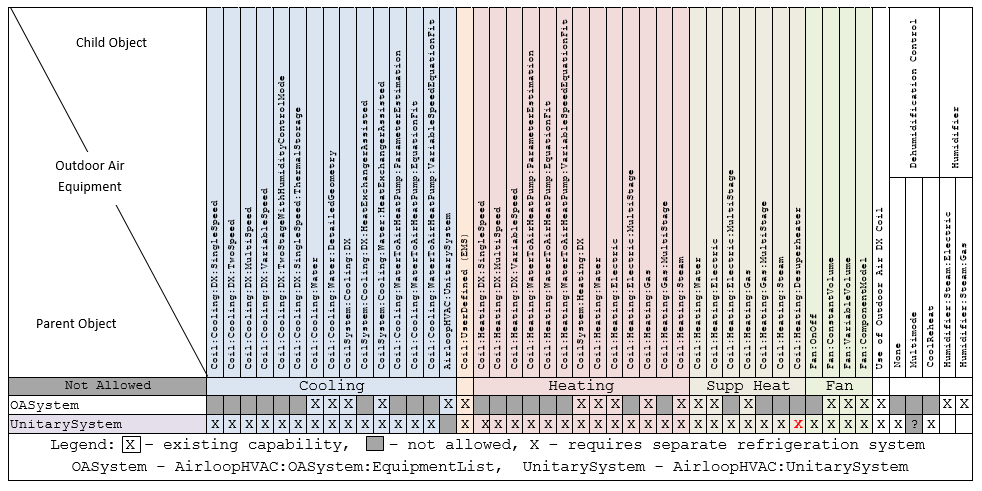
\includegraphics{media/OASysComponentMatrix.png}
\caption{Outdoor Air System Component Matrix \protect \label{fig:outdoor-air-system-component-matrix}}
\end{figure}

\subsubsection{Inputs}\label{inputs-4-001}

\paragraph{Field: Name}\label{field-name-4-001}

The user designated unique name of an instance of an Air Loop Equipment List. Any object referencing this Air Loop Equipment List will do so using this name.

\paragraph{Field Set (Component Object Type,, Component Name) up to 8}\label{field-set-component-object-type-component-name-up-to-8}

After the identifying name, the list consists of up to 8 pairs of data items:

\paragraph{Field: Component \textless{}x\textgreater{} Object Type}\label{field-component-x-object-type}

This field specifies the keyword for the type of component used.

\paragraph{Field: Component \textless{}x\textgreater{} Name}\label{field-component-x-name}

This field is the unique name of the component specified in the previous field. This named object must appear in the IDF.

An example from an IDF:

\begin{lstlisting}

AirLoopHVAC:OutdoorAirSystem:EquipmentList,
             OA Sys 1 Equipment,
             HeatExchanger:AirToAir:FlatPlate,OA Heat Recovery 1,
             OutdoorAir:Mixer, OA Mixing Box 1;
\end{lstlisting}

\subsection{OutdoorAir:Node}\label{outdoorairnode}

The OutdoorAir:Node object declares an HVAC system node for outdoor air conditions. The program automatically sets the air conditions at these nodes to correspond to the ambient environmental conditions at the beginning of every timestep. The outdoor air node is typically used as the inlet air node to an HVAC component such as the \hyperref[outdoorairmixer]{OutdoorAir:Mixer} object. Multiple OutdoorAir:Node objects can be used in an input file, however, duplicate node names are not allowed.

The \emph{Height Above Ground} field is used to adjust the weather file air conditions, e.g., outdoor dry-bulb and wet-bulb air temperatures, for atmospheric variation with height. This variation can become a significant factor when modeling tall buildings. See the Engineering Reference section on Atmospheric Variation for a description of the algorithm for variation of atmospheric properties with height. A blank entry or a value less than zero for this field indicates that the height will be ignored and the weather file conditions will be used.

\textbf{OutdoorAir:Node} and \textbf{\hyperref[outdoorairnodelist]{OutdoorAir:\hyperref[nodelist]{NodeList}}} both set a node to outdoor air conditions. \textbf{OutdoorAir:Node} modifies the weather file conditions if a height has been specified. \textbf{\hyperref[outdoorairnodelist]{OutdoorAir:\hyperref[nodelist]{NodeList}}} does not have a height input and always uses the weather file conditions without modification. The same node name may not be used with both of these objects.

When declared in surface property objects \textbf{\hyperref[surfacePropertylocalEnvironment]{SurfaceProperty:LocalEnvironment}}, in zone property objects \textbf{\hyperref[ZonePropertylocalEnvironment]{ZoneProperty:LocalEnvironment}}, or as an external node in the airflow network calculation linking to a surface node \textbf{AirflowNetwork:Multizone:Surface}, the object can also be used to define local outdoor air conditions for surfaces, zones or air loop components. The local outdoor air conditions would be used in the EnergyPlus calculations for:
\begin{enumerate}
\item Convection coefficients used in the exterior surface heat balance

If the user declares a local surface outdoor air node to overwrite the surface level environmental data, the convection coefficients would be calculated based on the local outdoor air node data accordingly based on surface level outdoor dry-bulb temperature, humidity ratio and wind speed.

\item Zone air infiltration and simple ventilation

If the user declares a local zone outdoor air node to overwrite zone level environmental data, global environmental variables used in the subroutines for infiltration and ventilation calculation, including outdoor air temperature, humidity ratio, enthalpy, wind speed and direction, would be overwritten accordingly with zone level data.

\item External air nodes used in the AirFlowNetwork

When used in the airflow network for wind pressure calculation, global environmental variables used in the subroutines for wind pressure calculation, including outdoor air temperature, humidity ratio, air density, wind speed and direction, would be overwritten accordingly with local data.

\end{enumerate}

When used in these cases, optional schedule inputs of local ambient air conditions, including dry-bulb temperature, wet-bulb temperature, wind velocity, and wind direction, can be defined in the optional fields. When used in the airflow network for wind pressure calculation, the wind pressure coefficient curve name and calculation details should also be defined.

\subsubsection{Inputs}\label{inputs-5-001}

\paragraph{Field: Name}\label{field-name-5-001}

The unique name for this outdoor air node.

\paragraph{Field: Height Above Ground}\label{field-height-above-ground}

The height {[}m{]} of the node above ground level. A value greater than zero allows the weather file conditions, e.g., outdoor dry-bulb and wet-bulb air temperatures, to be adjusted according to atmospheric variation with height.

A blank entry or value less than zero indicates that the height will be ignored and the weather file conditions will be used.

\paragraph{Field: Drybulb Temperature Schedule Name}\label{field-drybulb-temperature-schedule-name}

This field is used to supply a schedule name of the local dry bulb temperature of this node. When the field is left blank, global values would be used in calculation.

\paragraph{Field: Wetbulb Temperature Schedule Name}\label{field-wetbulb-temperature-schedule-name}

This field is used to supply a schedule name of the local wet bulb temperature of this node. When the field is left blank, global values would be used in calculation.

\paragraph{Field: Wind Speed Schedule Name}\label{field-wind-speed-schedule-name}

This field is used to supply a schedule name of the local wind speed of this node. When the field is left blank, global values would be used in calculation.

\paragraph{Field: Wind Direction Schedule Name}\label{field-wind-dir-schedule-name}

This field is used to supply a schedule name of the local wind direction of this node. When the field is left blank, global values would be used in calculation.

\paragraph{Field: Wind Pressure Coefficient Curve Name}\label{field-wind-pressure-coeff-curve-name}

The name of a specific \textbf{\hyperref[airflownetworkmultizonewindpressurecoefficientvalues]{AirflowNetwork:MultiZone:WindPressureCoefficientValues}} object (which gives wind pressure coefficients for the façade as a function of angle of wind incident on the façade).

\paragraph{Field: Symmetric Wind Pressure Coefficient Curve}\label{field-sym-windp-curve-name}

This field is used to specify whether the pressure curve is symmetric or not. \textbf{Yes} for curves that should be evaluated from 0 to 180 degrees. \textbf{No} for curves that should be evaluated from 0 to 360 degrees.

\paragraph{Field: Wind Angle Type}

This field is used to specify whether the angle used to compute the wind pressure coefficient is absolute or relative. \textbf{Relative} for computing the angle between the wind direction and the surface azimuth. \textbf{Absolute} for using the wind direction angle directly.

An example IDF:

\begin{lstlisting}

OutdoorAir:Node,
  OA Node 1;  !- Name

OutdoorAir:Node,
  Floor 10 Outdoor air Inlet Node,  !- Name
  30.0;  !- Height Above Ground {m}

OutdoorAir:Node,
  LocalOutdoorAirNode:0001,     !- Name
  ,                             !- Height Above Ground
  OutdoorAirNodeDryBulb:0001,   !- Drybulb Temperature Schedule Name
  OutdoorAirNodeWetBulb:0001,   !- Wetbulb Temperature Schedule Name
  OutdoorAirNodeWindSpeed:0001, !- Wind Speed Schedule Name
  OutdoorAirNodeWindDir:0001;   !- Wind Direction Schedule Name
  NFacade_WPCValue,             !- Wind Pressure Coefficient Curve Name
  No,                           !- Symmetric Wind Pressure Coefficient Curve
  Absolute;                     !- Wind Angle Type
\end{lstlisting}

\subsection{Outdoor Air Node outputs:}\label{outdoor-air-node-outputs}

The ambient dry-bulb, wet-bulb air temperature, wind speed and direction, and flow rate at the outdoor air node can be monitored using the system node output variables:

\begin{itemize}
\item
  HVAC,Average,System Node Temperature {[}C{]}
\item
  HVAC,Average,System Node Wetbulb Temperature {[}C{]}
\item
  HVAC,Average,System Node Wind Speed {[}m/s{]}
\item
  HVAC,Average,System Node Wind Direction {[}degree{]}
\item
  HVAC,Average,System Node Mass Flow Rate {[}kg/s{]}
\end{itemize}

e.g.

\begin{lstlisting}

Output:Variable,
  Floor 10 Outdoor air Inlet Node,
  System Node Temperature,
  Hourly;
\end{lstlisting}


\subsection{OutdoorAir:NodeList}\label{outdoorairnodelist}

The program needs to know which HVAC system nodes are inlets for outdoor air. Knowing this, the program can set the conditions at these nodes to the outdoor conditions at the start of each major timestep. The \hyperref[outdoorairnode]{OutdoorAir:Node}List provides the means for specifying which nodes are outdoor air nodes.

The input is flexible: there may be one or more \hyperref[outdoorairnode]{OutdoorAir:Node}List in each input file. Each list contains up to 25 names. The names can be the name of a unique HVAC system node, or the name of a Node List which will contain the actual node names. Duplicate node names are ignored.

\textbf{\hyperref[outdoorairnode]{OutdoorAir:Node}} and \textbf{\hyperref[outdoorairnode]{OutdoorAir:Node}List} both set a node to outdoor air conditions. \textbf{\hyperref[outdoorairnode]{OutdoorAir:Node}} modifies the weather file conditions if a height has been specified. \textbf{\hyperref[outdoorairnode]{OutdoorAir:Node}List} does not have a height input and always uses the weather file conditions without modification. The same node name may not be used with both of these objects.

\subsubsection{Inputs}\label{inputs-6-001}

\paragraph{Field: Node or NodeList name}\label{field-node-or-nodelist-name}

The name of an HVAC system node or of a \hyperref[nodelist]{NodeList} object. There can be up to 25 names.

An example IDF:

\begin{lstlisting}

OutdoorAir:NodeList,
      OutsideAirInletNodes;

  NodeList,OutsideAirInletNodes,
      Outdoor air Inlet Node;
\end{lstlisting}

\subsection{OutdoorAir:Mixer}\label{outdoorairmixer}

The OutdoorAir:Mixer is the most common component used in an outdoor air system. The outdoor air mixer has 2 inlet air streams: the system return air and the outdoor air. It has 2 outlet air streams: the system relief air and the mixed air. This is a passive component. It takes the inlet mass flows and conditions plus the relief air mass flow and calculates the mixed air flow rate and conditions (as well as the relief air conditions). The inlet and relief mass flow must be set outside the component -- most commonly by an outdoor air controller. The OutdoorAir:Mixer can also be used in compound components such as a fan coil unit.

Input for this object is very simple: a unique name plus the node names of the 2 inlet nodes and the 2 outlet nodes.

\subsubsection{Inputs}\label{inputs-7-001}

\paragraph{Field: Name}\label{field-name-6-001}

A unique user assigned name for a particular outdoor air mixer component. Any reference to this component by another object will use this name.

\paragraph{Field: Mixed Air Node Name}\label{field-mixed-air-node-name}

The name of the HVAC system node which is the outlet for the mixed air stream.

\paragraph{Field: Outdoor Air Stream Node Name}\label{field-outdoor-air-stream-node-name}

The name of the HVAC system node which is the inlet for the outdoor air stream.

\paragraph{Field: Relief Air Stream Node Name}\label{field-relief-air-stream-node-name}

The name of the HVAC system node which is the outlet for the system relief air.

\paragraph{Field: Return Air Stream Node Name}\label{field-return-air-stream-node-name}

The name of the HVAC system node which is the inlet for the return air stream.

An IDF example:

\begin{lstlisting}

OutdoorAir:Mixer,
      Zone1WindACOAMixer,           ! name
      Zone1WindACOAMixerOutletNode, ! mixer outlet node
      Zone1WindACOAInNode,          ! mixer OA node
      Zone1WindACExhNode,           ! mixer relief node
      Zone1WindACAirInletNode;      ! mixer inlet node
\end{lstlisting}
